% ============================================================
% ============================================================
% NACA0012 -- SURFACE TEMPERATURE AND FREEZING FRACTION
% ============================================================
% ============================================================


% ============================================================
% Surface Temperature -- Both Conditions
% ============================================================

\begin{frame}{\small NACA0012 -- Surface Temperature Comparison}
\scriptsize

\begin{columns}[T,onlytextwidth]

\begin{column}{0.50\textwidth}
    \centering
    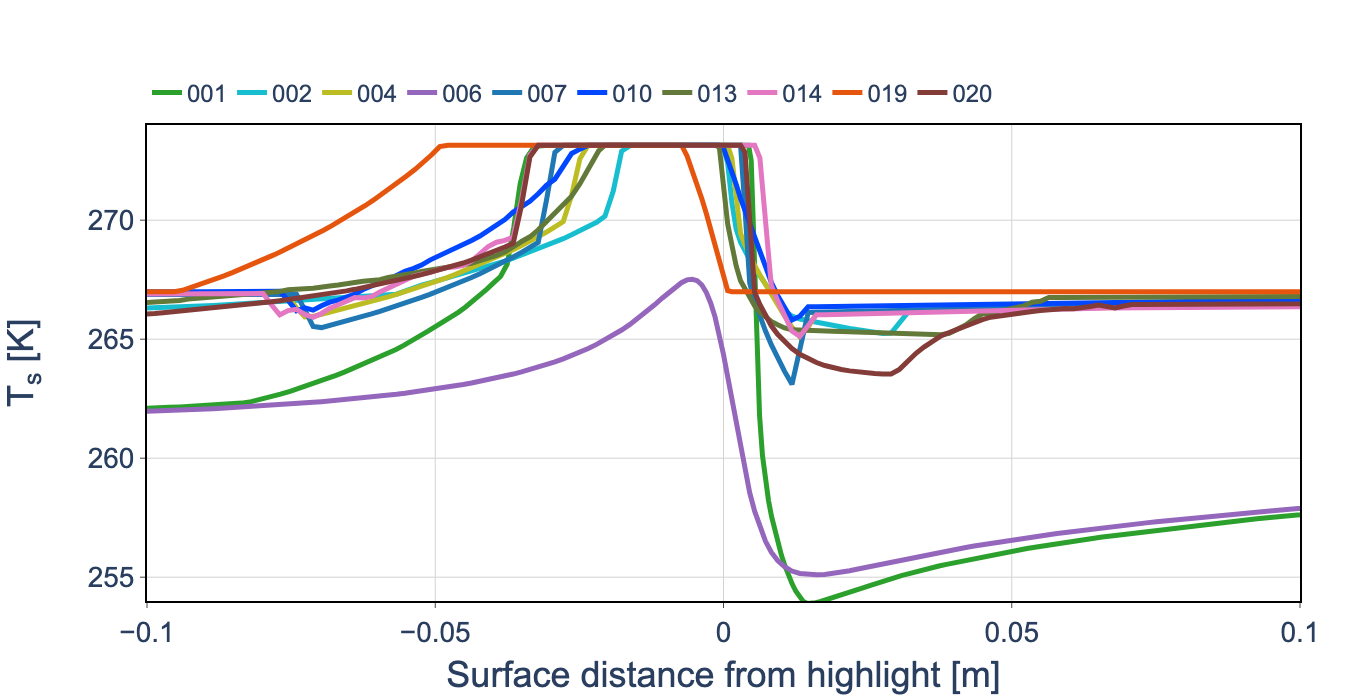
\includegraphics[width=\textwidth]{FIGURES/SURF_TEMP_FF/tc_naca0012_ae3932_L1_surface_temperature_vs_s_slice_0p9144_all_roughness.png}

    \vspace{0.05cm}

    {\scriptsize\textbf{AE3932}}
\end{column}

\begin{column}{0.50\textwidth}
    \centering
    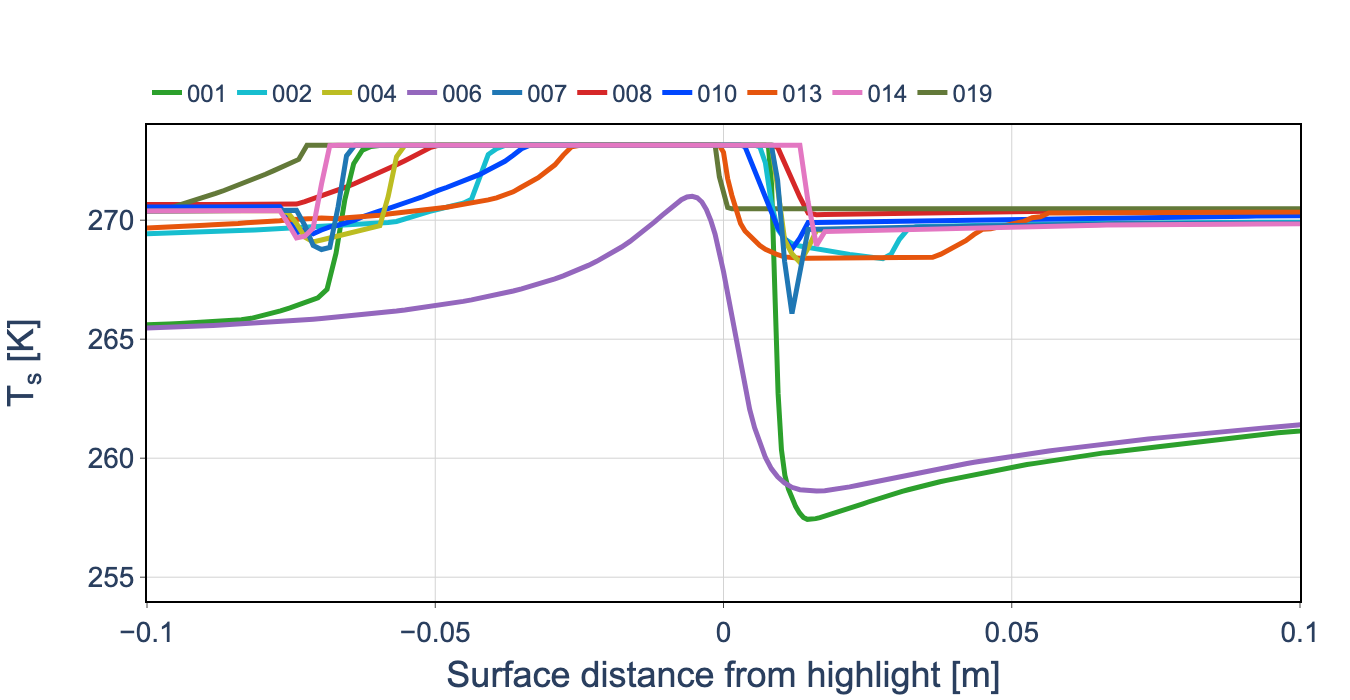
\includegraphics[width=\textwidth]{FIGURES/SURF_TEMP_FF/tc_naca0012_ae3933_L1_surface_temperature_vs_s_slice_0p9144_all_roughness.png}

    \vspace{0.05cm}

    {\scriptsize\textbf{AE3933}}
\end{column}

\end{columns}

\vspace{0.15cm}

\begin{block}{\scriptsize Observations}
\begin{itemize}
    \item Substantial code-to-code variability is observed in the surface-temperature distributions for both conditions.
    \item Differences between AE3932 and AE3933 are also evident in the predicted surface thermal response.
\end{itemize}
\end{block}

\end{frame}


% ============================================================
% Freezing Fraction -- Both Conditions
% ============================================================

\begin{frame}{\small NACA0012 -- Freezing Fraction Comparison}
\scriptsize

\begin{columns}[T,onlytextwidth]

\begin{column}{0.50\textwidth}
    \centering
    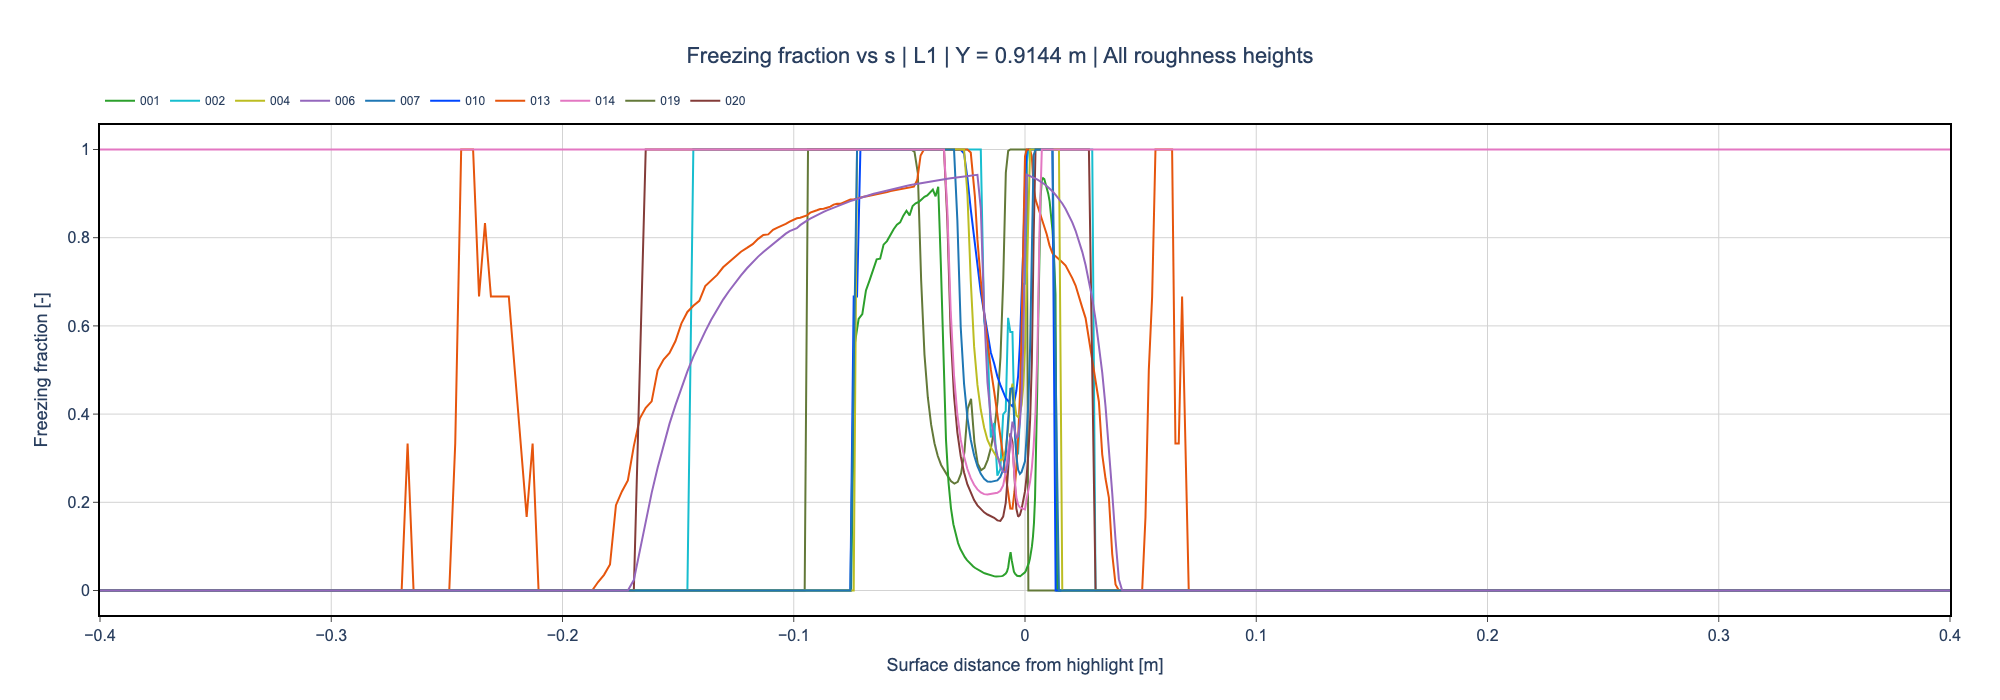
\includegraphics[width=\textwidth]{FIGURES/SURF_TEMP_FF/tc_naca0012_ae3932_L1_freezing_fraction_vs_s_slice_0p9144_all_roughness.png}

    \vspace{0.05cm}

    {\scriptsize\textbf{AE3932}}
\end{column}

\begin{column}{0.50\textwidth}
    \centering
    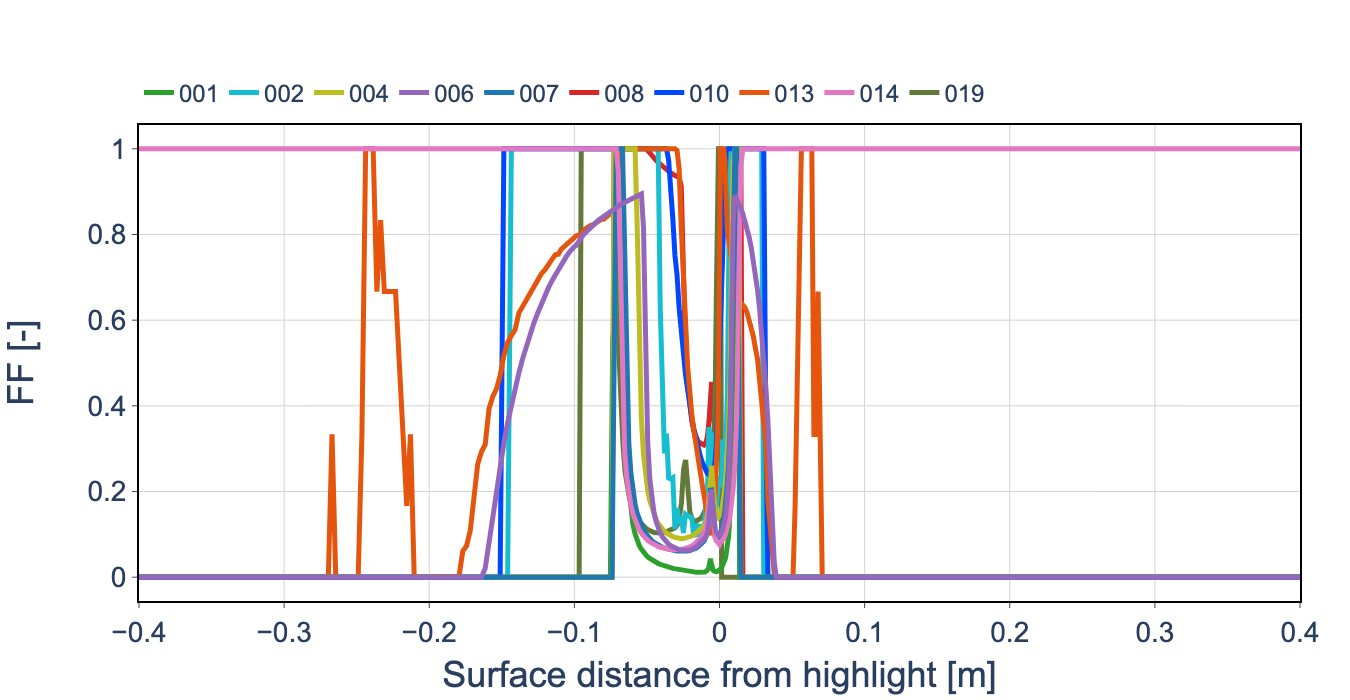
\includegraphics[width=\textwidth]{FIGURES/SURF_TEMP_FF/tc_naca0012_ae3933_L1_freezing_fraction_vs_s_slice_0p9144_all_roughness.png}

    \vspace{0.05cm}

    {\scriptsize\textbf{AE3933}}
\end{column}

\end{columns}

\vspace{0.15cm}

\begin{block}{\scriptsize Observations}
\begin{itemize}
    \item Considerable code-to-code variability is observed in the freezing fraction for both conditions.
    \item Different thermodynamic regimes and transition locations are predicted across submissions.
    \item Sharp and spatially shifted transitions make direct pointwise comparison particularly difficult.
\end{itemize}
\end{block}

\end{frame}

% ============================================================
% NACA0012 -- HTC & Thermodynamics Assessment
% ============================================================

\begin{frame}{\small NACA0012 -- HTC \& Thermodynamics Assessment}
\scriptsize

\begin{block}{\scriptsize Recovery Temperature}
\begin{itemize}
    \item Closely clustered across submissions, consistent with the good agreement in $C_p$.
\end{itemize}
\end{block}

\vspace{0.12cm}

\begin{block}{\scriptsize Convective Heat Transfer}
\begin{itemize}
    \item Larger code-to-code variability is observed in $HTC$ and $Q_c'$, with roughness explaining only part of the spread.
    \item Grid sensitivity remains comparatively limited for most submissions.
\end{itemize}
\end{block}

\vspace{0.12cm}

\begin{block}{\scriptsize Thermodynamic Response}
\begin{itemize}
    \item Surface temperature and freezing fraction exhibit substantial code-to-code variability.
    \item Different freezing regimes and transition locations are predicted across submissions.
\end{itemize}
\end{block}

\vspace{0.12cm}

\begin{alertblock}{\scriptsize Takeaway}
Aerodynamic agreement leads to consistent $T_{\mathrm{rec}}$, while larger differences emerge in $HTC$ and propagate into the predicted thermodynamic response.
\end{alertblock}

\end{frame}